\documentclass[1p]{elsarticle_modified}
%\bibliographystyle{elsarticle-num}

%\usepackage[colorlinks]{hyperref}
%\usepackage{abbrmath_seonhwa} %\Abb, \Ascr, \Acal ,\Abf, \Afrak
\usepackage{amsfonts}
\usepackage{amssymb}
\usepackage{amsmath}
\usepackage{amsthm}
\usepackage{scalefnt}
\usepackage{amsbsy}
\usepackage{kotex}
\usepackage{caption}
\usepackage{subfig}
\usepackage{color}
\usepackage{graphicx}
\usepackage{xcolor} %% white, black, red, green, blue, cyan, magenta, yellow
\usepackage{float}
\usepackage{setspace}
\usepackage{hyperref}

\usepackage{tikz}
\usetikzlibrary{arrows}

\usepackage{multirow}
\usepackage{array} % fixed length table
\usepackage{hhline}

%%%%%%%%%%%%%%%%%%%%%
\makeatletter
\renewcommand*\env@matrix[1][\arraystretch]{%
	\edef\arraystretch{#1}%
	\hskip -\arraycolsep
	\let\@ifnextchar\new@ifnextchar
	\array{*\c@MaxMatrixCols c}}
\makeatother %https://tex.stackexchange.com/questions/14071/how-can-i-increase-the-line-spacing-in-a-matrix
%%%%%%%%%%%%%%%

\usepackage[normalem]{ulem}

\newcommand{\msout}[1]{\ifmmode\text{\sout{\ensuremath{#1}}}\else\sout{#1}\fi}
%SOURCE: \msout is \stkout macro in https://tex.stackexchange.com/questions/20609/strikeout-in-math-mode

\newcommand{\cancel}[1]{
	\ifmmode
	{\color{red}\msout{#1}}
	\else
	{\color{red}\sout{#1}}
	\fi
}

\newcommand{\add}[1]{
	{\color{blue}\uwave{#1}}
}

\newcommand{\replace}[2]{
	\ifmmode
	{\color{red}\msout{#1}}{\color{blue}\uwave{#2}}
	\else
	{\color{red}\sout{#1}}{\color{blue}\uwave{#2}}
	\fi
}

\newcommand{\Sol}{\mathcal{S}} %segment
\newcommand{\D}{D} %diagram
\newcommand{\A}{\mathcal{A}} %arc


%%%%%%%%%%%%%%%%%%%%%%%%%%%%%5 test

\def\sl{\operatorname{\textup{SL}}(2,\Cbb)}
\def\psl{\operatorname{\textup{PSL}}(2,\Cbb)}
\def\quan{\mkern 1mu \triangleright \mkern 1mu}

\theoremstyle{definition}
\newtheorem{thm}{Theorem}[section]
\newtheorem{prop}[thm]{Proposition}
\newtheorem{lem}[thm]{Lemma}
\newtheorem{ques}[thm]{Question}
\newtheorem{cor}[thm]{Corollary}
\newtheorem{defn}[thm]{Definition}
\newtheorem{exam}[thm]{Example}
\newtheorem{rmk}[thm]{Remark}
\newtheorem{alg}[thm]{Algorithm}

\newcommand{\I}{\sqrt{-1}}
\begin{document}

%\begin{frontmatter}
%
%\title{Boundary parabolic representations of knots up to 8 crossings}
%
%%% Group authors per affiliation:
%\author{Yunhi Cho} 
%\address{Department of Mathematics, University of Seoul, Seoul, Korea}
%\ead{yhcho@uos.ac.kr}
%
%
%\author{Seonhwa Kim} %\fnref{s_kim}}
%\address{Center for Geometry and Physics, Institute for Basic Science, Pohang, 37673, Korea}
%\ead{ryeona17@ibs.re.kr}
%
%\author{Hyuk Kim}
%\address{Department of Mathematical Sciences, Seoul National University, Seoul 08826, Korea}
%\ead{hyukkim@snu.ac.kr}
%
%\author{Seokbeom Yoon}
%\address{Department of Mathematical Sciences, Seoul National University, Seoul, 08826,  Korea}
%\ead{sbyoon15@snu.ac.kr}
%
%\begin{abstract}
%We find all boundary parabolic representation of knots up to 8 crossings.
%
%\end{abstract}
%\begin{keyword}
%    \MSC[2010] 57M25 
%\end{keyword}
%
%\end{frontmatter}

%\linenumbers
%\tableofcontents
%
\newcommand\colored[1]{\textcolor{white}{\rule[-0.35ex]{0.8em}{1.4ex}}\kern-0.8em\color{red} #1}%
%\newcommand\colored[1]{\textcolor{white}{ #1}\kern-2.17ex	\textcolor{white}{ #1}\kern-1.81ex	\textcolor{white}{ #1}\kern-2.15ex\color{red}#1	}

{\Large $\underline{12a_{0559}~(K12a_{0559})}$}

\setlength{\tabcolsep}{10pt}
\renewcommand{\arraystretch}{1.6}
\vspace{1cm}\begin{tabular}{m{100pt}>{\centering\arraybackslash}m{274pt}}
\multirow{5}{120pt}{
	\centering
	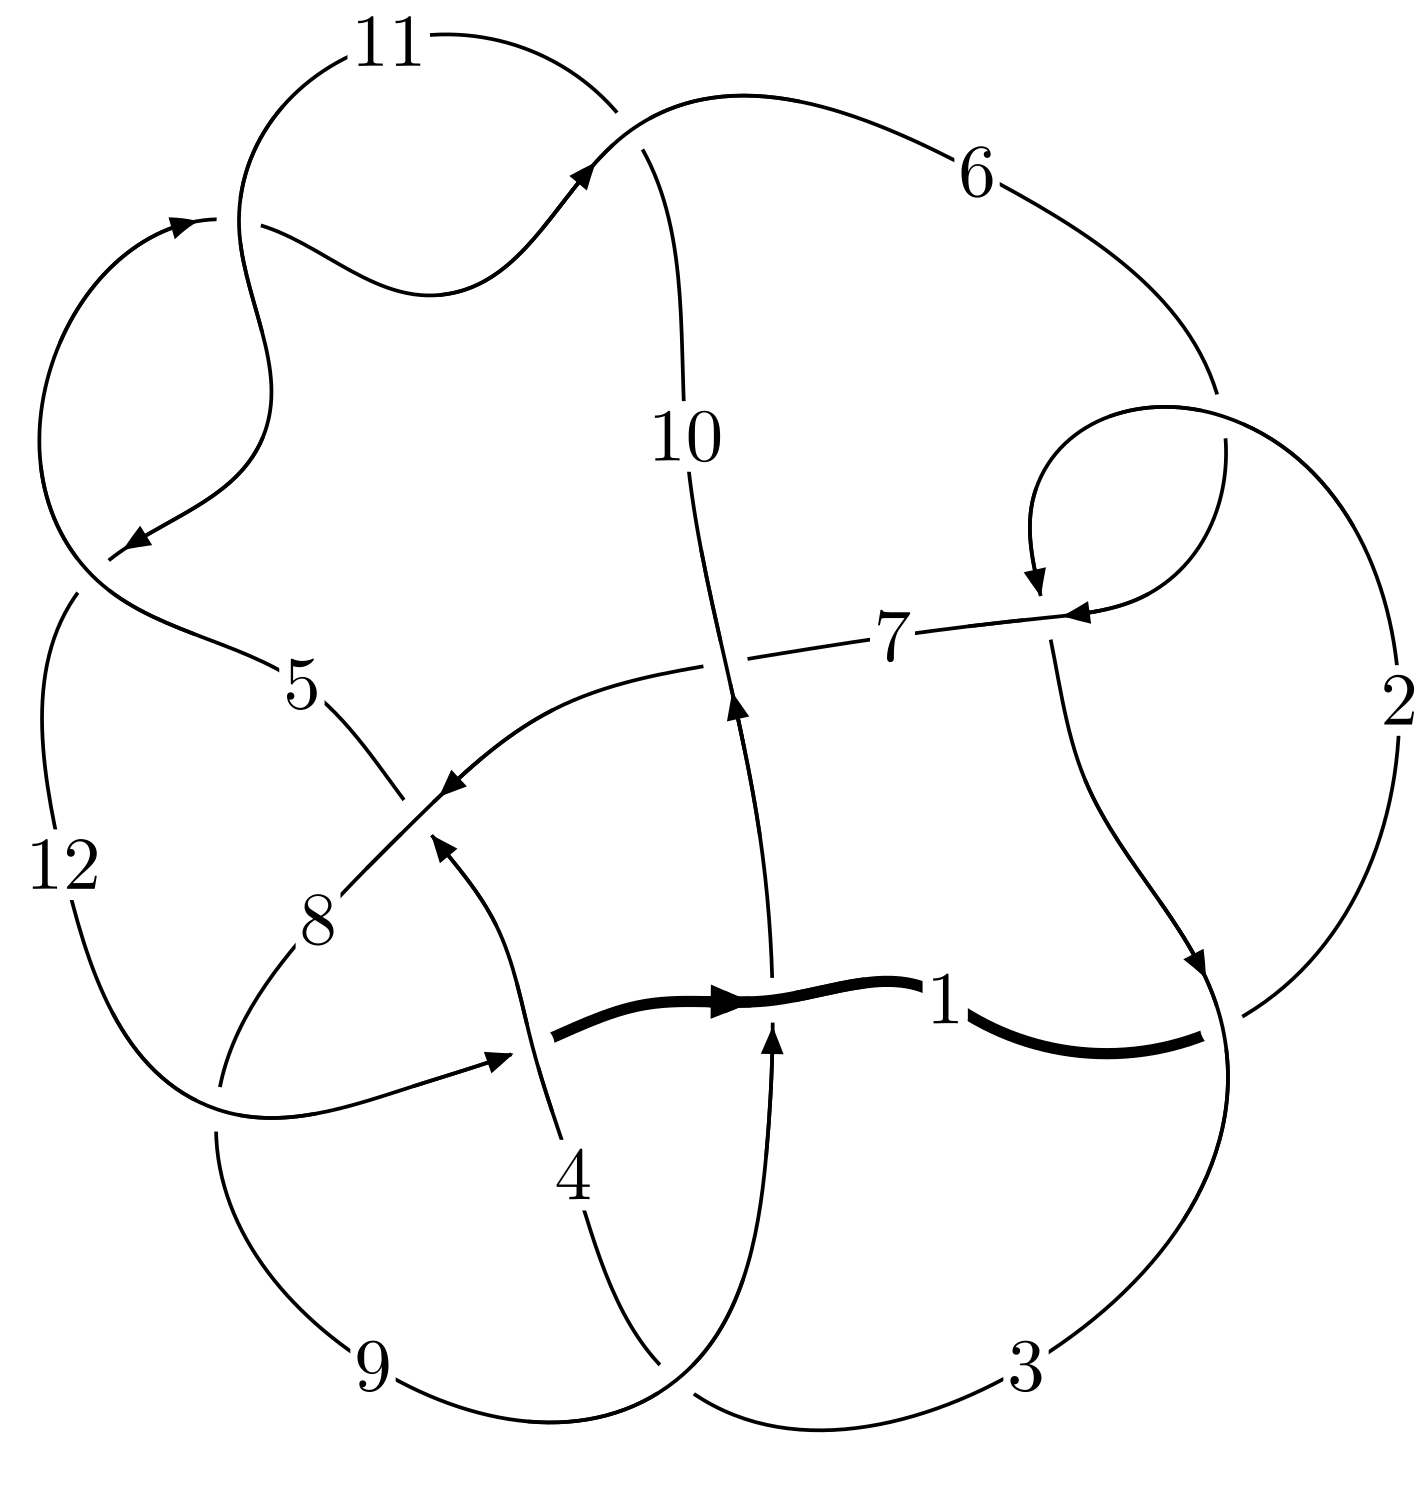
\includegraphics[width=112pt]{../../../GIT/diagram.site/Diagrams/png/1360_12a_0559.png}\\
\ \ \ A knot diagram\footnotemark}&
\allowdisplaybreaks
\textbf{Linearized knot diagam} \\
\cline{2-2}
 &
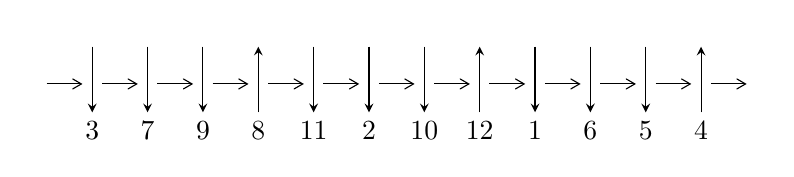
\begin{tikzpicture}[x=20pt, y=17pt]
	% nodes
	\node (C0) at (0, 0) {};
	\node (C1) at (1, 0) {};
	\node (C1U) at (1, +1) {};
	\node (C1D) at (1, -1) {3};

	\node (C2) at (2, 0) {};
	\node (C2U) at (2, +1) {};
	\node (C2D) at (2, -1) {7};

	\node (C3) at (3, 0) {};
	\node (C3U) at (3, +1) {};
	\node (C3D) at (3, -1) {9};

	\node (C4) at (4, 0) {};
	\node (C4U) at (4, +1) {};
	\node (C4D) at (4, -1) {8};

	\node (C5) at (5, 0) {};
	\node (C5U) at (5, +1) {};
	\node (C5D) at (5, -1) {11};

	\node (C6) at (6, 0) {};
	\node (C6U) at (6, +1) {};
	\node (C6D) at (6, -1) {2};

	\node (C7) at (7, 0) {};
	\node (C7U) at (7, +1) {};
	\node (C7D) at (7, -1) {10};

	\node (C8) at (8, 0) {};
	\node (C8U) at (8, +1) {};
	\node (C8D) at (8, -1) {12};

	\node (C9) at (9, 0) {};
	\node (C9U) at (9, +1) {};
	\node (C9D) at (9, -1) {1};

	\node (C10) at (10, 0) {};
	\node (C10U) at (10, +1) {};
	\node (C10D) at (10, -1) {6};

	\node (C11) at (11, 0) {};
	\node (C11U) at (11, +1) {};
	\node (C11D) at (11, -1) {5};

	\node (C12) at (12, 0) {};
	\node (C12U) at (12, +1) {};
	\node (C12D) at (12, -1) {4};
	\node (C13) at (13, 0) {};

	% arrows
	\draw[->,>={angle 60}]
	(C0) edge (C1) (C1) edge (C2) (C2) edge (C3) (C3) edge (C4) (C4) edge (C5) (C5) edge (C6) (C6) edge (C7) (C7) edge (C8) (C8) edge (C9) (C9) edge (C10) (C10) edge (C11) (C11) edge (C12) (C12) edge (C13) ;	\draw[->,>=stealth]
	(C1U) edge (C1D) (C2U) edge (C2D) (C3U) edge (C3D) (C4D) edge (C4U) (C5U) edge (C5D) (C6U) edge (C6D) (C7U) edge (C7D) (C8D) edge (C8U) (C9U) edge (C9D) (C10U) edge (C10D) (C11U) edge (C11D) (C12D) edge (C12U) ;
	\end{tikzpicture} \\
\hhline{~~} \\& 
\textbf{Solving Sequence} \\ \cline{2-2} 
 &
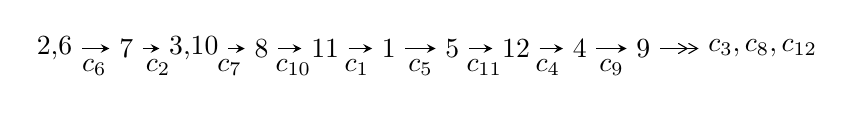
\begin{tikzpicture}[x=23pt, y=7pt]
	% node
	\node (A0) at (-1/8, 0) {2,6};
	\node (A1) at (1, 0) {7};
	\node (A2) at (33/16, 0) {3,10};
	\node (A3) at (25/8, 0) {8};
	\node (A4) at (33/8, 0) {11};
	\node (A5) at (41/8, 0) {1};
	\node (A6) at (49/8, 0) {5};
	\node (A7) at (57/8, 0) {12};
	\node (A8) at (65/8, 0) {4};
	\node (A9) at (73/8, 0) {9};
	\node (C1) at (1/2, -1) {$c_{6}$};
	\node (C2) at (3/2, -1) {$c_{2}$};
	\node (C3) at (21/8, -1) {$c_{7}$};
	\node (C4) at (29/8, -1) {$c_{10}$};
	\node (C5) at (37/8, -1) {$c_{1}$};
	\node (C6) at (45/8, -1) {$c_{5}$};
	\node (C7) at (53/8, -1) {$c_{11}$};
	\node (C8) at (61/8, -1) {$c_{4}$};
	\node (C9) at (69/8, -1) {$c_{9}$};
	\node (A10) at (11, 0) {$c_{3},c_{8},c_{12}$};

	% edge
	\draw[->,>=stealth]	
	(A0) edge (A1) (A1) edge (A2) (A2) edge (A3) (A3) edge (A4) (A4) edge (A5) (A5) edge (A6) (A6) edge (A7) (A7) edge (A8) (A8) edge (A9) ;
	\draw[->>,>={angle 60}]	
	(A9) edge (A10);
\end{tikzpicture} \\ 

\end{tabular} \\

\footnotetext{
The image of knot diagram is generated by the software ``\textbf{Draw programme}" developed by Andrew Bartholomew(\url{http://www.layer8.co.uk/maths/draw/index.htm\#Running-draw}), where we modified some parts for our purpose(\url{https://github.com/CATsTAILs/LinksPainter}).
}\phantom \\ \newline 
\centering \textbf{Ideals for irreducible components\footnotemark of $X_{\text{par}}$} 
 
\begin{align*}
I^u_{1}&=\langle 
-2.62320\times10^{287} u^{131}+4.40473\times10^{287} u^{130}+\cdots+3.61885\times10^{287} b+1.06624\times10^{289},\\
\phantom{I^u_{1}}&\phantom{= \langle  }-2.63834\times10^{289} u^{131}+5.53105\times10^{289} u^{130}+\cdots+3.22078\times10^{289} a+1.89383\times10^{291},\\
\phantom{I^u_{1}}&\phantom{= \langle  }u^{132}-2 u^{131}+\cdots-568 u+89\rangle \\
I^u_{2}&=\langle 
u^{26}+u^{25}+\cdots+b-3,\;u^{26}- u^{25}+\cdots+a-4,\;u^{27}- u^{26}+\cdots- u+1\rangle \\
\\
\end{align*}
\raggedright * 2 irreducible components of $\dim_{\mathbb{C}}=0$, with total 159 representations.\\
\footnotetext{All coefficients of polynomials are rational numbers. But the coefficients are sometimes approximated in decimal forms when there is not enough margin.}
\newpage
\renewcommand{\arraystretch}{1}
\centering \section*{I. $I^u_{1}= \langle -2.62\times10^{287} u^{131}+4.40\times10^{287} u^{130}+\cdots+3.62\times10^{287} b+1.07\times10^{289},\;-2.64\times10^{289} u^{131}+5.53\times10^{289} u^{130}+\cdots+3.22\times10^{289} a+1.89\times10^{291},\;u^{132}-2 u^{131}+\cdots-568 u+89 \rangle$}
\flushleft \textbf{(i) Arc colorings}\\
\begin{tabular}{m{7pt} m{180pt} m{7pt} m{180pt} }
\flushright $a_{2}=$&$\begin{pmatrix}0\\u\end{pmatrix}$ \\
\flushright $a_{6}=$&$\begin{pmatrix}1\\0\end{pmatrix}$ \\
\flushright $a_{7}=$&$\begin{pmatrix}1\\u^2\end{pmatrix}$ \\
\flushright $a_{3}=$&$\begin{pmatrix}- u\\- u^3+u\end{pmatrix}$ \\
\flushright $a_{10}=$&$\begin{pmatrix}0.819162 u^{131}-1.71730 u^{130}+\cdots-59.4863 u-58.8003\\0.724872 u^{131}-1.21716 u^{130}+\cdots+89.8247 u-29.4635\end{pmatrix}$ \\
\flushright $a_{8}=$&$\begin{pmatrix}-0.161670 u^{131}+0.565376 u^{130}+\cdots-192.959 u+20.9352\\-1.16897 u^{131}+1.80579 u^{130}+\cdots+227.476 u-27.4721\end{pmatrix}$ \\
\flushright $a_{11}=$&$\begin{pmatrix}0.0942905 u^{131}-0.500140 u^{130}+\cdots-149.311 u-29.3368\\0.724872 u^{131}-1.21716 u^{130}+\cdots+89.8247 u-29.4635\end{pmatrix}$ \\
\flushright $a_{1}=$&$\begin{pmatrix}u^3\\u^5- u^3+u\end{pmatrix}$ \\
\flushright $a_{5}=$&$\begin{pmatrix}-0.181553 u^{131}-1.14469 u^{130}+\cdots-695.765 u+80.9396\\-0.710908 u^{131}+2.82353 u^{130}+\cdots-208.303 u+36.9135\end{pmatrix}$ \\
\flushright $a_{12}=$&$\begin{pmatrix}0.785751 u^{131}+0.104849 u^{130}+\cdots-302.478 u-82.3601\\-3.50233 u^{131}+7.09633 u^{130}+\cdots+998.390 u-103.373\end{pmatrix}$ \\
\flushright $a_{4}=$&$\begin{pmatrix}0.203113 u^{131}-0.0820425 u^{130}+\cdots+102.209 u-54.2446\\-0.0191589 u^{131}+0.624928 u^{130}+\cdots+112.201 u-26.3748\end{pmatrix}$ \\
\flushright $a_{9}=$&$\begin{pmatrix}0.439066 u^{131}-1.19115 u^{130}+\cdots+406.652 u-120.893\\0.884407 u^{131}-1.78507 u^{130}+\cdots-213.423 u+18.7842\end{pmatrix}$\\&\end{tabular}
\flushleft \textbf{(ii) Obstruction class $= -1$}\\~\\
\flushleft \textbf{(iii) Cusp Shapes $= 8.49058 u^{131}-24.4730 u^{130}+\cdots+488.947 u-51.1479$}\\~\\
\newpage\renewcommand{\arraystretch}{1}
\flushleft \textbf{(iv) u-Polynomials at the component}\newline \\
\begin{tabular}{m{50pt}|m{274pt}}
Crossings & \hspace{64pt}u-Polynomials at each crossing \\
\hline $$\begin{aligned}c_{1}\end{aligned}$$&$\begin{aligned}
&u^{132}+50 u^{131}+\cdots+410734 u+7921
\end{aligned}$\\
\hline $$\begin{aligned}c_{2},c_{6}\end{aligned}$$&$\begin{aligned}
&u^{132}-2 u^{131}+\cdots-568 u+89
\end{aligned}$\\
\hline $$\begin{aligned}c_{3}\end{aligned}$$&$\begin{aligned}
&u^{132}-2 u^{131}+\cdots+29779 u+2021
\end{aligned}$\\
\hline $$\begin{aligned}c_{4}\end{aligned}$$&$\begin{aligned}
&u^{132}-6 u^{131}+\cdots-1890 u+251
\end{aligned}$\\
\hline $$\begin{aligned}c_{5},c_{10},c_{11}\end{aligned}$$&$\begin{aligned}
&u^{132}+u^{131}+\cdots+133 u+11
\end{aligned}$\\
\hline $$\begin{aligned}c_{7}\end{aligned}$$&$\begin{aligned}
&u^{132}+u^{131}+\cdots+3639368 u-287749
\end{aligned}$\\
\hline $$\begin{aligned}c_{8}\end{aligned}$$&$\begin{aligned}
&u^{132}-22 u^{130}+\cdots+185420 u+16129
\end{aligned}$\\
\hline $$\begin{aligned}c_{9}\end{aligned}$$&$\begin{aligned}
&u^{132}-5 u^{131}+\cdots-4 u-1
\end{aligned}$\\
\hline $$\begin{aligned}c_{12}\end{aligned}$$&$\begin{aligned}
&u^{132}+9 u^{131}+\cdots+72 u+11
\end{aligned}$\\
\hline
\end{tabular}\\~\\
\newpage\renewcommand{\arraystretch}{1}
\flushleft \textbf{(v) Riley Polynomials at the component}\newline \\
\begin{tabular}{m{50pt}|m{274pt}}
Crossings & \hspace{64pt}Riley Polynomials at each crossing \\
\hline $$\begin{aligned}c_{1}\end{aligned}$$&$\begin{aligned}
&y^{132}+74 y^{131}+\cdots-5025488686 y+62742241
\end{aligned}$\\
\hline $$\begin{aligned}c_{2},c_{6}\end{aligned}$$&$\begin{aligned}
&y^{132}-50 y^{131}+\cdots-410734 y+7921
\end{aligned}$\\
\hline $$\begin{aligned}c_{3}\end{aligned}$$&$\begin{aligned}
&y^{132}+28 y^{131}+\cdots-150607255 y+4084441
\end{aligned}$\\
\hline $$\begin{aligned}c_{4}\end{aligned}$$&$\begin{aligned}
&y^{132}-22 y^{131}+\cdots-2514888 y+63001
\end{aligned}$\\
\hline $$\begin{aligned}c_{5},c_{10},c_{11}\end{aligned}$$&$\begin{aligned}
&y^{132}+147 y^{131}+\cdots-40855 y+121
\end{aligned}$\\
\hline $$\begin{aligned}c_{7}\end{aligned}$$&$\begin{aligned}
&y^{132}+51 y^{131}+\cdots-2120861931094 y+82799487001
\end{aligned}$\\
\hline $$\begin{aligned}c_{8}\end{aligned}$$&$\begin{aligned}
&y^{132}-44 y^{131}+\cdots+4699377698 y+260144641
\end{aligned}$\\
\hline $$\begin{aligned}c_{9}\end{aligned}$$&$\begin{aligned}
&y^{132}-13 y^{131}+\cdots+8 y+1
\end{aligned}$\\
\hline $$\begin{aligned}c_{12}\end{aligned}$$&$\begin{aligned}
&y^{132}+27 y^{131}+\cdots+6476 y+121
\end{aligned}$\\
\hline
\end{tabular}\\~\\
\newpage\flushleft \textbf{(vi) Complex Volumes and Cusp Shapes}
$$\begin{array}{c|c|c}  
\text{Solutions to }I^u_{1}& \I (\text{vol} + \sqrt{-1}CS) & \text{Cusp shape}\\
 \hline 
\begin{aligned}
u &= \phantom{-}0.994996 + 0.006480 I \\
a &= -1.74092 - 0.54070 I \\
b &= -0.471730 - 0.131016 I\end{aligned}
 & -4.62550 - 1.48283 I & \phantom{-0.000000 } 0 \\ \hline\begin{aligned}
u &= \phantom{-}0.994996 - 0.006480 I \\
a &= -1.74092 + 0.54070 I \\
b &= -0.471730 + 0.131016 I\end{aligned}
 & -4.62550 + 1.48283 I & \phantom{-0.000000 } 0 \\ \hline\begin{aligned}
u &= \phantom{-}0.634066 + 0.801263 I \\
a &= \phantom{-}0.634491 + 0.575872 I \\
b &= \phantom{-}0.13578 - 1.45796 I\end{aligned}
 & \phantom{-}6.19734 + 4.07644 I & \phantom{-0.000000 } 0 \\ \hline\begin{aligned}
u &= \phantom{-}0.634066 - 0.801263 I \\
a &= \phantom{-}0.634491 - 0.575872 I \\
b &= \phantom{-}0.13578 + 1.45796 I\end{aligned}
 & \phantom{-}6.19734 - 4.07644 I & \phantom{-0.000000 } 0 \\ \hline\begin{aligned}
u &= \phantom{-}0.515731 + 0.831149 I \\
a &= \phantom{-}0.404778 - 0.164401 I \\
b &= \phantom{-}0.051469 - 0.567679 I\end{aligned}
 & \phantom{-}3.79838 + 2.24121 I & \phantom{-0.000000 } 0 \\ \hline\begin{aligned}
u &= \phantom{-}0.515731 - 0.831149 I \\
a &= \phantom{-}0.404778 + 0.164401 I \\
b &= \phantom{-}0.051469 + 0.567679 I\end{aligned}
 & \phantom{-}3.79838 - 2.24121 I & \phantom{-0.000000 } 0 \\ \hline\begin{aligned}
u &= -0.752149 + 0.624524 I \\
a &= \phantom{-}1.90916 + 0.67170 I \\
b &= \phantom{-}0.034547 - 0.281824 I\end{aligned}
 & \phantom{-}2.55140 - 1.93292 I & \phantom{-0.000000 } 0 \\ \hline\begin{aligned}
u &= -0.752149 - 0.624524 I \\
a &= \phantom{-}1.90916 - 0.67170 I \\
b &= \phantom{-}0.034547 + 0.281824 I\end{aligned}
 & \phantom{-}2.55140 + 1.93292 I & \phantom{-0.000000 } 0 \\ \hline\begin{aligned}
u &= -0.668759 + 0.711722 I \\
a &= \phantom{-}0.808567 + 0.081701 I \\
b &= \phantom{-}0.589563 + 0.305614 I\end{aligned}
 & \phantom{-}0.48044 - 1.66584 I & \phantom{-0.000000 } 0 \\ \hline\begin{aligned}
u &= -0.668759 - 0.711722 I \\
a &= \phantom{-}0.808567 - 0.081701 I \\
b &= \phantom{-}0.589563 - 0.305614 I\end{aligned}
 & \phantom{-}0.48044 + 1.66584 I & \phantom{-0.000000 } 0\\
 \hline 
 \end{array}$$\newpage$$\begin{array}{c|c|c}  
\text{Solutions to }I^u_{1}& \I (\text{vol} + \sqrt{-1}CS) & \text{Cusp shape}\\
 \hline 
\begin{aligned}
u &= -0.570024 + 0.863514 I \\
a &= -0.222453 - 0.052071 I \\
b &= -0.734101 - 0.708592 I\end{aligned}
 & \phantom{-}2.59743 - 8.93120 I & \phantom{-0.000000 } 0 \\ \hline\begin{aligned}
u &= -0.570024 - 0.863514 I \\
a &= -0.222453 + 0.052071 I \\
b &= -0.734101 + 0.708592 I\end{aligned}
 & \phantom{-}2.59743 + 8.93120 I & \phantom{-0.000000 } 0 \\ \hline\begin{aligned}
u &= -0.360635 + 0.971464 I \\
a &= -0.0362939 - 0.0413371 I \\
b &= -0.403332 + 0.366839 I\end{aligned}
 & \phantom{-}1.52321 + 4.62993 I & \phantom{-0.000000 } 0 \\ \hline\begin{aligned}
u &= -0.360635 - 0.971464 I \\
a &= -0.0362939 + 0.0413371 I \\
b &= -0.403332 - 0.366839 I\end{aligned}
 & \phantom{-}1.52321 - 4.62993 I & \phantom{-0.000000 } 0 \\ \hline\begin{aligned}
u &= -0.904663 + 0.509921 I \\
a &= -0.826665 - 0.848051 I \\
b &= -0.535360 - 0.451714 I\end{aligned}
 & -1.89833 + 2.87175 I & \phantom{-0.000000 } 0 \\ \hline\begin{aligned}
u &= -0.904663 - 0.509921 I \\
a &= -0.826665 + 0.848051 I \\
b &= -0.535360 + 0.451714 I\end{aligned}
 & -1.89833 - 2.87175 I & \phantom{-0.000000 } 0 \\ \hline\begin{aligned}
u &= \phantom{-}0.784767 + 0.682639 I \\
a &= \phantom{-}1.132960 - 0.122173 I \\
b &= \phantom{-}0.413696 + 0.801010 I\end{aligned}
 & \phantom{-}1.94520 - 2.06908 I & \phantom{-0.000000 } 0 \\ \hline\begin{aligned}
u &= \phantom{-}0.784767 - 0.682639 I \\
a &= \phantom{-}1.132960 + 0.122173 I \\
b &= \phantom{-}0.413696 - 0.801010 I\end{aligned}
 & \phantom{-}1.94520 + 2.06908 I & \phantom{-0.000000 } 0 \\ \hline\begin{aligned}
u &= \phantom{-}0.819759 + 0.645897 I \\
a &= -0.39488 - 1.50469 I \\
b &= \phantom{-}0.01450 + 1.53948 I\end{aligned}
 & \phantom{-}8.87156 - 6.85147 I & \phantom{-0.000000 } 0 \\ \hline\begin{aligned}
u &= \phantom{-}0.819759 - 0.645897 I \\
a &= -0.39488 + 1.50469 I \\
b &= \phantom{-}0.01450 - 1.53948 I\end{aligned}
 & \phantom{-}8.87156 + 6.85147 I & \phantom{-0.000000 } 0\\
 \hline 
 \end{array}$$\newpage$$\begin{array}{c|c|c}  
\text{Solutions to }I^u_{1}& \I (\text{vol} + \sqrt{-1}CS) & \text{Cusp shape}\\
 \hline 
\begin{aligned}
u &= -0.822814 + 0.646545 I \\
a &= -1.53339 - 0.88035 I \\
b &= -0.966960 + 0.552965 I\end{aligned}
 & \phantom{-}3.07535 + 5.04428 I & \phantom{-0.000000 } 0 \\ \hline\begin{aligned}
u &= -0.822814 - 0.646545 I \\
a &= -1.53339 + 0.88035 I \\
b &= -0.966960 - 0.552965 I\end{aligned}
 & \phantom{-}3.07535 - 5.04428 I & \phantom{-0.000000 } 0 \\ \hline\begin{aligned}
u &= \phantom{-}0.565290 + 0.765188 I \\
a &= \phantom{-}0.054701 + 0.324447 I \\
b &= -0.693226 + 0.744308 I\end{aligned}
 & \phantom{-}4.10966 + 0.92164 I & \phantom{-0.000000 } 0 \\ \hline\begin{aligned}
u &= \phantom{-}0.565290 - 0.765188 I \\
a &= \phantom{-}0.054701 - 0.324447 I \\
b &= -0.693226 - 0.744308 I\end{aligned}
 & \phantom{-}4.10966 - 0.92164 I & \phantom{-0.000000 } 0 \\ \hline\begin{aligned}
u &= -1.04902\phantom{ +0.000000I} \\
a &= \phantom{-}1.07199\phantom{ +0.000000I} \\
b &= \phantom{-}0.691178\phantom{ +0.000000I}\end{aligned}
 & -1.61809\phantom{ +0.000000I} & \phantom{-0.000000 } 0 \\ \hline\begin{aligned}
u &= \phantom{-}0.868569 + 0.386574 I \\
a &= -1.76217 + 0.96278 I \\
b &= -0.172034 - 0.799347 I\end{aligned}
 & -2.84775 - 1.60335 I & \phantom{-0.000000 } 0 \\ \hline\begin{aligned}
u &= \phantom{-}0.868569 - 0.386574 I \\
a &= -1.76217 - 0.96278 I \\
b &= -0.172034 + 0.799347 I\end{aligned}
 & -2.84775 + 1.60335 I & \phantom{-0.000000 } 0 \\ \hline\begin{aligned}
u &= \phantom{-}0.772456 + 0.715664 I \\
a &= \phantom{-}0.742267 - 0.744997 I \\
b &= -0.067281 + 0.621184 I\end{aligned}
 & \phantom{-}2.35190 - 2.68342 I & \phantom{-0.000000 } 0 \\ \hline\begin{aligned}
u &= \phantom{-}0.772456 - 0.715664 I \\
a &= \phantom{-}0.742267 + 0.744997 I \\
b &= -0.067281 - 0.621184 I\end{aligned}
 & \phantom{-}2.35190 + 2.68342 I & \phantom{-0.000000 } 0 \\ \hline\begin{aligned}
u &= \phantom{-}0.771908 + 0.729236 I \\
a &= -0.053680 + 0.255973 I \\
b &= \phantom{-}0.26793 - 1.61185 I\end{aligned}
 & \phantom{-}10.54430 + 4.25109 I & \phantom{-0.000000 } 0\\
 \hline 
 \end{array}$$\newpage$$\begin{array}{c|c|c}  
\text{Solutions to }I^u_{1}& \I (\text{vol} + \sqrt{-1}CS) & \text{Cusp shape}\\
 \hline 
\begin{aligned}
u &= \phantom{-}0.771908 - 0.729236 I \\
a &= -0.053680 - 0.255973 I \\
b &= \phantom{-}0.26793 + 1.61185 I\end{aligned}
 & \phantom{-}10.54430 - 4.25109 I & \phantom{-0.000000 } 0 \\ \hline\begin{aligned}
u &= -1.064160 + 0.060889 I \\
a &= \phantom{-}1.55659 - 0.12062 I \\
b &= \phantom{-}0.771807 - 0.677807 I\end{aligned}
 & -3.49156 - 2.47310 I & \phantom{-0.000000 } 0 \\ \hline\begin{aligned}
u &= -1.064160 - 0.060889 I \\
a &= \phantom{-}1.55659 + 0.12062 I \\
b &= \phantom{-}0.771807 + 0.677807 I\end{aligned}
 & -3.49156 + 2.47310 I & \phantom{-0.000000 } 0 \\ \hline\begin{aligned}
u &= -0.857199 + 0.640093 I \\
a &= -1.009080 - 0.133591 I \\
b &= \phantom{-}0.25723 + 1.85429 I\end{aligned}
 & \phantom{-}7.67912 + 1.97784 I & \phantom{-0.000000 } 0 \\ \hline\begin{aligned}
u &= -0.857199 - 0.640093 I \\
a &= -1.009080 + 0.133591 I \\
b &= \phantom{-}0.25723 - 1.85429 I\end{aligned}
 & \phantom{-}7.67912 - 1.97784 I & \phantom{-0.000000 } 0 \\ \hline\begin{aligned}
u &= -0.856401 + 0.642335 I \\
a &= -2.13306 - 0.42776 I \\
b &= -0.36336 + 1.80298 I\end{aligned}
 & \phantom{-}7.68137 + 3.02430 I & \phantom{-0.000000 } 0 \\ \hline\begin{aligned}
u &= -0.856401 - 0.642335 I \\
a &= -2.13306 + 0.42776 I \\
b &= -0.36336 - 1.80298 I\end{aligned}
 & \phantom{-}7.68137 - 3.02430 I & \phantom{-0.000000 } 0 \\ \hline\begin{aligned}
u &= -0.880379 + 0.638494 I \\
a &= \phantom{-}0.436321 + 0.517027 I \\
b &= \phantom{-}0.885433 + 0.705363 I\end{aligned}
 & \phantom{-}2.89468 - 0.02986 I & \phantom{-0.000000 } 0 \\ \hline\begin{aligned}
u &= -0.880379 - 0.638494 I \\
a &= \phantom{-}0.436321 - 0.517027 I \\
b &= \phantom{-}0.885433 - 0.705363 I\end{aligned}
 & \phantom{-}2.89468 + 0.02986 I & \phantom{-0.000000 } 0 \\ \hline\begin{aligned}
u &= -1.069670 + 0.201549 I \\
a &= -0.918165 - 1.030270 I \\
b &= -0.356229 - 0.381280 I\end{aligned}
 & -3.90078 - 0.34266 I & \phantom{-0.000000 } 0\\
 \hline 
 \end{array}$$\newpage$$\begin{array}{c|c|c}  
\text{Solutions to }I^u_{1}& \I (\text{vol} + \sqrt{-1}CS) & \text{Cusp shape}\\
 \hline 
\begin{aligned}
u &= -1.069670 - 0.201549 I \\
a &= -0.918165 + 1.030270 I \\
b &= -0.356229 + 0.381280 I\end{aligned}
 & -3.90078 + 0.34266 I & \phantom{-0.000000 } 0 \\ \hline\begin{aligned}
u &= \phantom{-}0.883959 + 0.638258 I \\
a &= \phantom{-}0.454032 - 0.216708 I \\
b &= \phantom{-}0.022800 + 0.763237 I\end{aligned}
 & \phantom{-}2.08747 - 2.56816 I & \phantom{-0.000000 } 0 \\ \hline\begin{aligned}
u &= \phantom{-}0.883959 - 0.638258 I \\
a &= \phantom{-}0.454032 + 0.216708 I \\
b &= \phantom{-}0.022800 - 0.763237 I\end{aligned}
 & \phantom{-}2.08747 + 2.56816 I & \phantom{-0.000000 } 0 \\ \hline\begin{aligned}
u &= -1.090650 + 0.093406 I \\
a &= -1.14572 + 1.64113 I \\
b &= -0.099797 + 1.342850 I\end{aligned}
 & -0.01929 + 3.49571 I & \phantom{-0.000000 } 0 \\ \hline\begin{aligned}
u &= -1.090650 - 0.093406 I \\
a &= -1.14572 - 1.64113 I \\
b &= -0.099797 - 1.342850 I\end{aligned}
 & -0.01929 - 3.49571 I & \phantom{-0.000000 } 0 \\ \hline\begin{aligned}
u &= \phantom{-}0.893330 + 0.649841 I \\
a &= \phantom{-}2.99081 - 0.53235 I \\
b &= \phantom{-}0.00730 + 1.48977 I\end{aligned}
 & \phantom{-}8.63942 + 1.80321 I & \phantom{-0.000000 } 0 \\ \hline\begin{aligned}
u &= \phantom{-}0.893330 - 0.649841 I \\
a &= \phantom{-}2.99081 + 0.53235 I \\
b &= \phantom{-}0.00730 - 1.48977 I\end{aligned}
 & \phantom{-}8.63942 - 1.80321 I & \phantom{-0.000000 } 0 \\ \hline\begin{aligned}
u &= -0.791276 + 0.772968 I \\
a &= \phantom{-}0.534673 + 0.705186 I \\
b &= -0.00970 - 1.58542 I\end{aligned}
 & \phantom{-}10.14180 + 2.60358 I & \phantom{-0.000000 } 0 \\ \hline\begin{aligned}
u &= -0.791276 - 0.772968 I \\
a &= \phantom{-}0.534673 - 0.705186 I \\
b &= -0.00970 + 1.58542 I\end{aligned}
 & \phantom{-}10.14180 - 2.60358 I & \phantom{-0.000000 } 0 \\ \hline\begin{aligned}
u &= \phantom{-}0.610674 + 0.649425 I \\
a &= -0.793420 + 1.044120 I \\
b &= -0.990122 - 0.247008 I\end{aligned}
 & \phantom{-}1.23734 + 3.50615 I & \phantom{-0.000000 } 0\\
 \hline 
 \end{array}$$\newpage$$\begin{array}{c|c|c}  
\text{Solutions to }I^u_{1}& \I (\text{vol} + \sqrt{-1}CS) & \text{Cusp shape}\\
 \hline 
\begin{aligned}
u &= \phantom{-}0.610674 - 0.649425 I \\
a &= -0.793420 - 1.044120 I \\
b &= -0.990122 + 0.247008 I\end{aligned}
 & \phantom{-}1.23734 - 3.50615 I & \phantom{-0.000000 } 0 \\ \hline\begin{aligned}
u &= -0.940716 + 0.613817 I \\
a &= -0.712349 + 0.771670 I \\
b &= -0.042375 - 0.473375 I\end{aligned}
 & \phantom{-}1.95733 + 6.81025 I & \phantom{-0.000000 } 0 \\ \hline\begin{aligned}
u &= -0.940716 - 0.613817 I \\
a &= -0.712349 - 0.771670 I \\
b &= -0.042375 + 0.473375 I\end{aligned}
 & \phantom{-}1.95733 - 6.81025 I & \phantom{-0.000000 } 0 \\ \hline\begin{aligned}
u &= \phantom{-}0.916598 + 0.667748 I \\
a &= -0.090668 + 0.660853 I \\
b &= -0.399787 + 0.923608 I\end{aligned}
 & \phantom{-}1.54193 - 3.15243 I & \phantom{-0.000000 } 0 \\ \hline\begin{aligned}
u &= \phantom{-}0.916598 - 0.667748 I \\
a &= -0.090668 - 0.660853 I \\
b &= -0.399787 - 0.923608 I\end{aligned}
 & \phantom{-}1.54193 + 3.15243 I & \phantom{-0.000000 } 0 \\ \hline\begin{aligned}
u &= -1.060320 + 0.411733 I \\
a &= \phantom{-}0.725968 + 0.184398 I \\
b &= \phantom{-}0.561074 - 0.066298 I\end{aligned}
 & -1.75667 + 0.49068 I & \phantom{-0.000000 } 0 \\ \hline\begin{aligned}
u &= -1.060320 - 0.411733 I \\
a &= \phantom{-}0.725968 - 0.184398 I \\
b &= \phantom{-}0.561074 + 0.066298 I\end{aligned}
 & -1.75667 - 0.49068 I & \phantom{-0.000000 } 0 \\ \hline\begin{aligned}
u &= -0.862337 + 0.746269 I \\
a &= \phantom{-}1.10193 + 1.14638 I \\
b &= \phantom{-}0.01425 - 1.58401 I\end{aligned}
 & \phantom{-}9.98298 + 2.82606 I & \phantom{-0.000000 } 0 \\ \hline\begin{aligned}
u &= -0.862337 - 0.746269 I \\
a &= \phantom{-}1.10193 - 1.14638 I \\
b &= \phantom{-}0.01425 + 1.58401 I\end{aligned}
 & \phantom{-}9.98298 - 2.82606 I & \phantom{-0.000000 } 0 \\ \hline\begin{aligned}
u &= \phantom{-}0.618325 + 0.966155 I \\
a &= -0.151389 - 0.572052 I \\
b &= -0.24136 + 1.59831 I\end{aligned}
 & \phantom{-}10.2195 + 12.5934 I & \phantom{-0.000000 } 0\\
 \hline 
 \end{array}$$\newpage$$\begin{array}{c|c|c}  
\text{Solutions to }I^u_{1}& \I (\text{vol} + \sqrt{-1}CS) & \text{Cusp shape}\\
 \hline 
\begin{aligned}
u &= \phantom{-}0.618325 - 0.966155 I \\
a &= -0.151389 + 0.572052 I \\
b &= -0.24136 - 1.59831 I\end{aligned}
 & \phantom{-}10.2195 - 12.5934 I & \phantom{-0.000000 } 0 \\ \hline\begin{aligned}
u &= -0.848464 + 0.077844 I \\
a &= -0.21096 + 3.29126 I \\
b &= -0.16663 + 1.42045 I\end{aligned}
 & \phantom{-}5.59934 + 5.71675 I & \phantom{-0.000000 } 0 \\ \hline\begin{aligned}
u &= -0.848464 - 0.077844 I \\
a &= -0.21096 - 3.29126 I \\
b &= -0.16663 - 1.42045 I\end{aligned}
 & \phantom{-}5.59934 - 5.71675 I & \phantom{-0.000000 } 0 \\ \hline\begin{aligned}
u &= \phantom{-}1.005330 + 0.564689 I \\
a &= -1.77666 + 0.33734 I \\
b &= -0.559377 - 0.541615 I\end{aligned}
 & -1.62372 - 6.68253 I & \phantom{-0.000000 } 0 \\ \hline\begin{aligned}
u &= \phantom{-}1.005330 - 0.564689 I \\
a &= -1.77666 - 0.33734 I \\
b &= -0.559377 + 0.541615 I\end{aligned}
 & -1.62372 + 6.68253 I & \phantom{-0.000000 } 0 \\ \hline\begin{aligned}
u &= -0.816595 + 0.161996 I \\
a &= -2.65788 + 0.25450 I \\
b &= -0.145940 + 1.183650 I\end{aligned}
 & -1.54149 + 0.68168 I & \phantom{-0.000000 } 0 \\ \hline\begin{aligned}
u &= -0.816595 - 0.161996 I \\
a &= -2.65788 - 0.25450 I \\
b &= -0.145940 - 1.183650 I\end{aligned}
 & -1.54149 - 0.68168 I & \phantom{-0.000000 } 0 \\ \hline\begin{aligned}
u &= \phantom{-}0.935862 + 0.699498 I \\
a &= -2.21328 + 0.14497 I \\
b &= -0.32179 - 1.57803 I\end{aligned}
 & \phantom{-}10.04390 - 9.70702 I & \phantom{-0.000000 } 0 \\ \hline\begin{aligned}
u &= \phantom{-}0.935862 - 0.699498 I \\
a &= -2.21328 - 0.14497 I \\
b &= -0.32179 + 1.57803 I\end{aligned}
 & \phantom{-}10.04390 + 9.70702 I & \phantom{-0.000000 } 0 \\ \hline\begin{aligned}
u &= -0.634146 + 0.985622 I \\
a &= \phantom{-}0.084459 + 0.505395 I \\
b &= -0.22551 - 1.58250 I\end{aligned}
 & \phantom{-}11.70150 - 4.34034 I & \phantom{-0.000000 } 0\\
 \hline 
 \end{array}$$\newpage$$\begin{array}{c|c|c}  
\text{Solutions to }I^u_{1}& \I (\text{vol} + \sqrt{-1}CS) & \text{Cusp shape}\\
 \hline 
\begin{aligned}
u &= -0.634146 - 0.985622 I \\
a &= \phantom{-}0.084459 - 0.505395 I \\
b &= -0.22551 + 1.58250 I\end{aligned}
 & \phantom{-}11.70150 + 4.34034 I & \phantom{-0.000000 } 0 \\ \hline\begin{aligned}
u &= -0.920415 + 0.726208 I \\
a &= \phantom{-}1.75168 + 0.54157 I \\
b &= \phantom{-}0.04906 - 1.54453 I\end{aligned}
 & \phantom{-}9.75071 + 3.05257 I & \phantom{-0.000000 } 0 \\ \hline\begin{aligned}
u &= -0.920415 - 0.726208 I \\
a &= \phantom{-}1.75168 - 0.54157 I \\
b &= \phantom{-}0.04906 + 1.54453 I\end{aligned}
 & \phantom{-}9.75071 - 3.05257 I & \phantom{-0.000000 } 0 \\ \hline\begin{aligned}
u &= -0.550360 + 1.043380 I \\
a &= \phantom{-}0.058196 - 0.472313 I \\
b &= \phantom{-}0.01923 + 1.53496 I\end{aligned}
 & \phantom{-}10.84940 - 2.52048 I & \phantom{-0.000000 } 0 \\ \hline\begin{aligned}
u &= -0.550360 - 1.043380 I \\
a &= \phantom{-}0.058196 + 0.472313 I \\
b &= \phantom{-}0.01923 - 1.53496 I\end{aligned}
 & \phantom{-}10.84940 + 2.52048 I & \phantom{-0.000000 } 0 \\ \hline\begin{aligned}
u &= \phantom{-}1.186540 + 0.094281 I \\
a &= \phantom{-}1.322460 + 0.412756 I \\
b &= \phantom{-}0.747039 + 0.446078 I\end{aligned}
 & -4.08907 - 7.51792 I & \phantom{-0.000000 } 0 \\ \hline\begin{aligned}
u &= \phantom{-}1.186540 - 0.094281 I \\
a &= \phantom{-}1.322460 - 0.412756 I \\
b &= \phantom{-}0.747039 - 0.446078 I\end{aligned}
 & -4.08907 + 7.51792 I & \phantom{-0.000000 } 0 \\ \hline\begin{aligned}
u &= \phantom{-}1.008060 + 0.637246 I \\
a &= \phantom{-}0.699716 - 0.829854 I \\
b &= \phantom{-}1.100490 - 0.415405 I\end{aligned}
 & \phantom{-}0.07070 - 8.57861 I & \phantom{-0.000000 } 0 \\ \hline\begin{aligned}
u &= \phantom{-}1.008060 - 0.637246 I \\
a &= \phantom{-}0.699716 + 0.829854 I \\
b &= \phantom{-}1.100490 + 0.415405 I\end{aligned}
 & \phantom{-}0.07070 + 8.57861 I & \phantom{-0.000000 } 0 \\ \hline\begin{aligned}
u &= -0.992211 + 0.669153 I \\
a &= -1.41520 - 0.58729 I \\
b &= -0.634108 + 0.248789 I\end{aligned}
 & -0.48526 + 6.98577 I & \phantom{-0.000000 } 0\\
 \hline 
 \end{array}$$\newpage$$\begin{array}{c|c|c}  
\text{Solutions to }I^u_{1}& \I (\text{vol} + \sqrt{-1}CS) & \text{Cusp shape}\\
 \hline 
\begin{aligned}
u &= -0.992211 - 0.669153 I \\
a &= -1.41520 + 0.58729 I \\
b &= -0.634108 - 0.248789 I\end{aligned}
 & -0.48526 - 6.98577 I & \phantom{-0.000000 } 0 \\ \hline\begin{aligned}
u &= \phantom{-}0.363034 + 0.711070 I \\
a &= \phantom{-}0.578080 - 0.413653 I \\
b &= -0.04916 + 1.43592 I\end{aligned}
 & \phantom{-}4.69090 - 1.42629 I & \phantom{-0.000000 } 0 \\ \hline\begin{aligned}
u &= \phantom{-}0.363034 - 0.711070 I \\
a &= \phantom{-}0.578080 + 0.413653 I \\
b &= -0.04916 - 1.43592 I\end{aligned}
 & \phantom{-}4.69090 + 1.42629 I & \phantom{-0.000000 } 0 \\ \hline\begin{aligned}
u &= \phantom{-}0.728610 + 0.293527 I \\
a &= \phantom{-}0.902833 + 0.437624 I \\
b &= \phantom{-}0.417664 - 0.606910 I\end{aligned}
 & -0.22605 + 2.50968 I & \phantom{-0.000000 } 0 \\ \hline\begin{aligned}
u &= \phantom{-}0.728610 - 0.293527 I \\
a &= \phantom{-}0.902833 - 0.437624 I \\
b &= \phantom{-}0.417664 + 0.606910 I\end{aligned}
 & -0.22605 - 2.50968 I & \phantom{-0.000000 } 0 \\ \hline\begin{aligned}
u &= \phantom{-}0.194079 + 1.201040 I \\
a &= -0.121857 + 0.524657 I \\
b &= -0.11940 - 1.48554 I\end{aligned}
 & \phantom{-}7.67886 - 6.48707 I & \phantom{-0.000000 } 0 \\ \hline\begin{aligned}
u &= \phantom{-}0.194079 - 1.201040 I \\
a &= -0.121857 - 0.524657 I \\
b &= -0.11940 + 1.48554 I\end{aligned}
 & \phantom{-}7.67886 + 6.48707 I & \phantom{-0.000000 } 0 \\ \hline\begin{aligned}
u &= \phantom{-}1.125170 + 0.465251 I \\
a &= \phantom{-}1.112720 + 0.521304 I \\
b &= \phantom{-}0.209271 + 1.325500 I\end{aligned}
 & \phantom{-}2.42090 - 3.32864 I & \phantom{-0.000000 } 0 \\ \hline\begin{aligned}
u &= \phantom{-}1.125170 - 0.465251 I \\
a &= \phantom{-}1.112720 - 0.521304 I \\
b &= \phantom{-}0.209271 - 1.325500 I\end{aligned}
 & \phantom{-}2.42090 + 3.32864 I & \phantom{-0.000000 } 0 \\ \hline\begin{aligned}
u &= -1.056440 + 0.608885 I \\
a &= -2.47896 + 0.30344 I \\
b &= -0.16650 + 1.54399 I\end{aligned}
 & \phantom{-}5.32474 + 9.30599 I & \phantom{-0.000000 } 0\\
 \hline 
 \end{array}$$\newpage$$\begin{array}{c|c|c}  
\text{Solutions to }I^u_{1}& \I (\text{vol} + \sqrt{-1}CS) & \text{Cusp shape}\\
 \hline 
\begin{aligned}
u &= -1.056440 - 0.608885 I \\
a &= -2.47896 - 0.30344 I \\
b &= -0.16650 - 1.54399 I\end{aligned}
 & \phantom{-}5.32474 - 9.30599 I & \phantom{-0.000000 } 0 \\ \hline\begin{aligned}
u &= \phantom{-}1.207290 + 0.185289 I \\
a &= -0.02766 + 1.65031 I \\
b &= -0.08721 + 1.50203 I\end{aligned}
 & \phantom{-}2.40715 + 1.84212 I & \phantom{-0.000000 } 0 \\ \hline\begin{aligned}
u &= \phantom{-}1.207290 - 0.185289 I \\
a &= -0.02766 - 1.65031 I \\
b &= -0.08721 - 1.50203 I\end{aligned}
 & \phantom{-}2.40715 - 1.84212 I & \phantom{-0.000000 } 0 \\ \hline\begin{aligned}
u &= \phantom{-}1.037550 + 0.662023 I \\
a &= \phantom{-}1.35614 - 0.48994 I \\
b &= \phantom{-}0.924834 + 0.683729 I\end{aligned}
 & \phantom{-}2.72984 - 6.32741 I & \phantom{-0.000000 } 0 \\ \hline\begin{aligned}
u &= \phantom{-}1.037550 - 0.662023 I \\
a &= \phantom{-}1.35614 + 0.48994 I \\
b &= \phantom{-}0.924834 - 0.683729 I\end{aligned}
 & \phantom{-}2.72984 + 6.32741 I & \phantom{-0.000000 } 0 \\ \hline\begin{aligned}
u &= -0.959303 + 0.789163 I \\
a &= -0.397598 - 0.522486 I \\
b &= -0.101230 + 0.195264 I\end{aligned}
 & -0.18630 + 3.08030 I & \phantom{-0.000000 } 0 \\ \hline\begin{aligned}
u &= -0.959303 - 0.789163 I \\
a &= -0.397598 + 0.522486 I \\
b &= -0.101230 - 0.195264 I\end{aligned}
 & -0.18630 - 3.08030 I & \phantom{-0.000000 } 0 \\ \hline\begin{aligned}
u &= \phantom{-}1.030710 + 0.697830 I \\
a &= -2.42414 + 0.08943 I \\
b &= -0.17012 - 1.44439 I\end{aligned}
 & \phantom{-}5.00651 - 9.72305 I & \phantom{-0.000000 } 0 \\ \hline\begin{aligned}
u &= \phantom{-}1.030710 - 0.697830 I \\
a &= -2.42414 - 0.08943 I \\
b &= -0.17012 + 1.44439 I\end{aligned}
 & \phantom{-}5.00651 + 9.72305 I & \phantom{-0.000000 } 0 \\ \hline\begin{aligned}
u &= \phantom{-}0.716992 + 0.124023 I \\
a &= \phantom{-}0.92913 + 2.53825 I \\
b &= -0.23110 + 1.45080 I\end{aligned}
 & \phantom{-}5.15288 - 0.10023 I & \phantom{-0.000000 } 0\\
 \hline 
 \end{array}$$\newpage$$\begin{array}{c|c|c}  
\text{Solutions to }I^u_{1}& \I (\text{vol} + \sqrt{-1}CS) & \text{Cusp shape}\\
 \hline 
\begin{aligned}
u &= \phantom{-}0.716992 - 0.124023 I \\
a &= \phantom{-}0.92913 - 2.53825 I \\
b &= -0.23110 - 1.45080 I\end{aligned}
 & \phantom{-}5.15288 + 0.10023 I & \phantom{-0.000000 } 0 \\ \hline\begin{aligned}
u &= \phantom{-}1.083560 + 0.675466 I \\
a &= -1.100260 - 0.103386 I \\
b &= -0.230811 - 0.496578 I\end{aligned}
 & \phantom{-}2.11983 - 7.86879 I & \phantom{-0.000000 } 0 \\ \hline\begin{aligned}
u &= \phantom{-}1.083560 - 0.675466 I \\
a &= -1.100260 + 0.103386 I \\
b &= -0.230811 + 0.496578 I\end{aligned}
 & \phantom{-}2.11983 + 7.86879 I & \phantom{-0.000000 } 0 \\ \hline\begin{aligned}
u &= -1.074050 + 0.695541 I \\
a &= \phantom{-}1.46630 + 0.54550 I \\
b &= \phantom{-}0.834487 - 0.713525 I\end{aligned}
 & \phantom{-}1.0717 + 14.7171 I & \phantom{-0.000000 } 0 \\ \hline\begin{aligned}
u &= -1.074050 - 0.695541 I \\
a &= \phantom{-}1.46630 - 0.54550 I \\
b &= \phantom{-}0.834487 + 0.713525 I\end{aligned}
 & \phantom{-}1.0717 - 14.7171 I & \phantom{-0.000000 } 0 \\ \hline\begin{aligned}
u &= -1.28440\phantom{ +0.000000I} \\
a &= -0.185699\phantom{ +0.000000I} \\
b &= \phantom{-}0.0492019\phantom{ +0.000000I}\end{aligned}
 & -2.37235\phantom{ +0.000000I} & \phantom{-0.000000 } 0 \\ \hline\begin{aligned}
u &= \phantom{-}0.676925 + 0.208900 I \\
a &= \phantom{-}1.124060 + 0.811472 I \\
b &= \phantom{-}0.04493 + 1.65565 I\end{aligned}
 & \phantom{-}5.40133 - 1.09492 I & \phantom{-0.000000 } 0 \\ \hline\begin{aligned}
u &= \phantom{-}0.676925 - 0.208900 I \\
a &= \phantom{-}1.124060 - 0.811472 I \\
b &= \phantom{-}0.04493 - 1.65565 I\end{aligned}
 & \phantom{-}5.40133 + 1.09492 I & \phantom{-0.000000 } 0 \\ \hline\begin{aligned}
u &= -1.280300 + 0.220518 I \\
a &= \phantom{-}0.983356 - 0.977949 I \\
b &= \phantom{-}0.23398 - 1.48521 I\end{aligned}
 & \phantom{-}2.15856 + 11.02100 I & \phantom{-0.000000 } 0 \\ \hline\begin{aligned}
u &= -1.280300 - 0.220518 I \\
a &= \phantom{-}0.983356 + 0.977949 I \\
b &= \phantom{-}0.23398 + 1.48521 I\end{aligned}
 & \phantom{-}2.15856 - 11.02100 I & \phantom{-0.000000 } 0\\
 \hline 
 \end{array}$$\newpage$$\begin{array}{c|c|c}  
\text{Solutions to }I^u_{1}& \I (\text{vol} + \sqrt{-1}CS) & \text{Cusp shape}\\
 \hline 
\begin{aligned}
u &= -0.348525 + 0.590263 I \\
a &= \phantom{-}0.771766 - 0.351389 I \\
b &= \phantom{-}0.12831 + 1.55884 I\end{aligned}
 & \phantom{-}7.05598 - 4.45947 I & -6.00000 + 2.49012 I \\ \hline\begin{aligned}
u &= -0.348525 - 0.590263 I \\
a &= \phantom{-}0.771766 + 0.351389 I \\
b &= \phantom{-}0.12831 - 1.55884 I\end{aligned}
 & \phantom{-}7.05598 + 4.45947 I & -6.00000 - 2.49012 I \\ \hline\begin{aligned}
u &= \phantom{-}1.101350 + 0.749789 I \\
a &= \phantom{-}1.95655 - 0.19479 I \\
b &= \phantom{-}0.27540 + 1.60963 I\end{aligned}
 & \phantom{-}8.7049 - 18.8638 I & \phantom{-0.000000 } 0 \\ \hline\begin{aligned}
u &= \phantom{-}1.101350 - 0.749789 I \\
a &= \phantom{-}1.95655 + 0.19479 I \\
b &= \phantom{-}0.27540 - 1.60963 I\end{aligned}
 & \phantom{-}8.7049 + 18.8638 I & \phantom{-0.000000 } 0 \\ \hline\begin{aligned}
u &= -1.095040 + 0.762225 I \\
a &= \phantom{-}1.72771 + 0.19647 I \\
b &= \phantom{-}0.28314 - 1.60368 I\end{aligned}
 & \phantom{-}10.2481 + 10.6947 I & \phantom{-0.000000 } 0 \\ \hline\begin{aligned}
u &= -1.095040 - 0.762225 I \\
a &= \phantom{-}1.72771 - 0.19647 I \\
b &= \phantom{-}0.28314 + 1.60368 I\end{aligned}
 & \phantom{-}10.2481 - 10.6947 I & \phantom{-0.000000 } 0 \\ \hline\begin{aligned}
u &= -0.526860 + 0.369790 I \\
a &= \phantom{-}1.258800 - 0.534568 I \\
b &= \phantom{-}0.12425 + 1.56373 I\end{aligned}
 & \phantom{-}7.07452 - 4.51449 I & -8.15922 + 1.95555 I \\ \hline\begin{aligned}
u &= -0.526860 - 0.369790 I \\
a &= \phantom{-}1.258800 + 0.534568 I \\
b &= \phantom{-}0.12425 - 1.56373 I\end{aligned}
 & \phantom{-}7.07452 + 4.51449 I & -8.15922 - 1.95555 I \\ \hline\begin{aligned}
u &= \phantom{-}1.000410 + 0.919179 I \\
a &= -0.958444 + 0.741591 I \\
b &= -0.02560 - 1.46902 I\end{aligned}
 & \phantom{-}5.55658 - 3.49041 I & \phantom{-0.000000 } 0 \\ \hline\begin{aligned}
u &= \phantom{-}1.000410 - 0.919179 I \\
a &= -0.958444 - 0.741591 I \\
b &= -0.02560 + 1.46902 I\end{aligned}
 & \phantom{-}5.55658 + 3.49041 I & \phantom{-0.000000 } 0\\
 \hline 
 \end{array}$$\newpage$$\begin{array}{c|c|c}  
\text{Solutions to }I^u_{1}& \I (\text{vol} + \sqrt{-1}CS) & \text{Cusp shape}\\
 \hline 
\begin{aligned}
u &= -1.154000 + 0.753313 I \\
a &= -1.55954 + 0.09926 I \\
b &= -0.07285 + 1.52892 I\end{aligned}
 & \phantom{-}8.95938 + 8.99501 I & \phantom{-0.000000 } 0 \\ \hline\begin{aligned}
u &= -1.154000 - 0.753313 I \\
a &= -1.55954 - 0.09926 I \\
b &= -0.07285 - 1.52892 I\end{aligned}
 & \phantom{-}8.95938 - 8.99501 I & \phantom{-0.000000 } 0 \\ \hline\begin{aligned}
u &= \phantom{-}1.150290 + 0.779742 I \\
a &= \phantom{-}0.933928 - 0.190095 I \\
b &= \phantom{-}0.236000 + 1.223090 I\end{aligned}
 & \phantom{-}2.04431 - 3.59566 I & \phantom{-0.000000 } 0 \\ \hline\begin{aligned}
u &= \phantom{-}1.150290 - 0.779742 I \\
a &= \phantom{-}0.933928 + 0.190095 I \\
b &= \phantom{-}0.236000 - 1.223090 I\end{aligned}
 & \phantom{-}2.04431 + 3.59566 I & \phantom{-0.000000 } 0 \\ \hline\begin{aligned}
u &= \phantom{-}0.338566 + 0.442940 I \\
a &= \phantom{-}0.892402 - 0.007273 I \\
b &= \phantom{-}0.447394 - 0.581047 I\end{aligned}
 & -0.14721 + 2.37366 I & -6.39573 - 4.68155 I \\ \hline\begin{aligned}
u &= \phantom{-}0.338566 - 0.442940 I \\
a &= \phantom{-}0.892402 + 0.007273 I \\
b &= \phantom{-}0.447394 + 0.581047 I\end{aligned}
 & -0.14721 - 2.37366 I & -6.39573 + 4.68155 I \\ \hline\begin{aligned}
u &= \phantom{-}1.43728 + 0.21546 I \\
a &= -0.377583 - 0.812593 I \\
b &= \phantom{-}0.04929 - 1.42523 I\end{aligned}
 & \phantom{-}2.52245 + 0.50257 I & \phantom{-0.000000 } 0 \\ \hline\begin{aligned}
u &= \phantom{-}1.43728 - 0.21546 I \\
a &= -0.377583 + 0.812593 I \\
b &= \phantom{-}0.04929 + 1.42523 I\end{aligned}
 & \phantom{-}2.52245 - 0.50257 I & \phantom{-0.000000 } 0 \\ \hline\begin{aligned}
u &= -0.316533 + 0.351504 I \\
a &= \phantom{-}1.022650 - 0.014973 I \\
b &= \phantom{-}0.404679 - 0.316331 I\end{aligned}
 & -0.902307 + 0.691481 I & -8.09755 - 4.83373 I \\ \hline\begin{aligned}
u &= -0.316533 - 0.351504 I \\
a &= \phantom{-}1.022650 + 0.014973 I \\
b &= \phantom{-}0.404679 + 0.316331 I\end{aligned}
 & -0.902307 - 0.691481 I & -8.09755 + 4.83373 I\\
 \hline 
 \end{array}$$\newpage$$\begin{array}{c|c|c}  
\text{Solutions to }I^u_{1}& \I (\text{vol} + \sqrt{-1}CS) & \text{Cusp shape}\\
 \hline 
\begin{aligned}
u &= \phantom{-}0.314071 + 0.042498 I \\
a &= -0.89991 + 4.02084 I \\
b &= -0.572934 + 0.019706 I\end{aligned}
 & \phantom{-}0.75055 + 3.16921 I & -9.99878 - 2.77340 I \\ \hline\begin{aligned}
u &= \phantom{-}0.314071 - 0.042498 I \\
a &= -0.89991 - 4.02084 I \\
b &= -0.572934 - 0.019706 I\end{aligned}
 & \phantom{-}0.75055 - 3.16921 I & -9.99878 + 2.77340 I\\
 \hline 
 \end{array}$$\newpage\newpage\renewcommand{\arraystretch}{1}
\centering \section*{II. $I^u_{2}= \langle u^{26}+u^{25}+\cdots+b-3,\;u^{26}- u^{25}+\cdots+a-4,\;u^{27}- u^{26}+\cdots- u+1 \rangle$}
\flushleft \textbf{(i) Arc colorings}\\
\begin{tabular}{m{7pt} m{180pt} m{7pt} m{180pt} }
\flushright $a_{2}=$&$\begin{pmatrix}0\\u\end{pmatrix}$ \\
\flushright $a_{6}=$&$\begin{pmatrix}1\\0\end{pmatrix}$ \\
\flushright $a_{7}=$&$\begin{pmatrix}1\\u^2\end{pmatrix}$ \\
\flushright $a_{3}=$&$\begin{pmatrix}- u\\- u^3+u\end{pmatrix}$ \\
\flushright $a_{10}=$&$\begin{pmatrix}- u^{26}+u^{25}+\cdots-4 u+4\\- u^{26}- u^{25}+\cdots+3 u+3\end{pmatrix}$ \\
\flushright $a_{8}=$&$\begin{pmatrix}3 u^{26}-2 u^{25}+\cdots+5 u-5\\-2 u^{26}+16 u^{24}+\cdots+8 u-6\end{pmatrix}$ \\
\flushright $a_{11}=$&$\begin{pmatrix}2 u^{25}-3 u^{24}+\cdots-7 u+1\\- u^{26}- u^{25}+\cdots+3 u+3\end{pmatrix}$ \\
\flushright $a_{1}=$&$\begin{pmatrix}u^3\\u^5- u^3+u\end{pmatrix}$ \\
\flushright $a_{5}=$&$\begin{pmatrix}-5 u^{26}+6 u^{25}+\cdots+11 u-2\\5 u^{26}-3 u^{25}+\cdots-5 u+3\end{pmatrix}$ \\
\flushright $a_{12}=$&$\begin{pmatrix}2 u^{26}+5 u^{25}+\cdots-2 u-5\\u^{24}-6 u^{23}+\cdots+u-9\end{pmatrix}$ \\
\flushright $a_{4}=$&$\begin{pmatrix}- u^{26}-2 u^{25}+\cdots+6 u+4\\4 u^{26}-3 u^{25}+\cdots+4 u-2\end{pmatrix}$ \\
\flushright $a_{9}=$&$\begin{pmatrix}- u^{26}+6 u^{24}+\cdots-4 u+4\\- u^{26}- u^{25}+\cdots+3 u+3\end{pmatrix}$\\&\end{tabular}
\flushleft \textbf{(ii) Obstruction class $= 1$}\\~\\
\flushleft \textbf{(iii) Cusp Shapes $= 20 u^{26}-23 u^{25}-108 u^{24}+147 u^{23}+321 u^{22}-491 u^{21}-648 u^{20}+1098 u^{19}+896 u^{18}-1787 u^{17}-859 u^{16}+2244 u^{15}+445 u^{14}-2209 u^{13}+114 u^{12}+1728 u^{11}-459 u^{10}-1053 u^9+524 u^8+485 u^7-354 u^6-145 u^5+176 u^4+22 u^3-62 u^2+15 u+9$}\\~\\
\newpage\renewcommand{\arraystretch}{1}
\flushleft \textbf{(iv) u-Polynomials at the component}\newline \\
\begin{tabular}{m{50pt}|m{274pt}}
Crossings & \hspace{64pt}u-Polynomials at each crossing \\
\hline $$\begin{aligned}c_{1}\end{aligned}$$&$\begin{aligned}
&u^{27}-13 u^{26}+\cdots+9 u-1
\end{aligned}$\\
\hline $$\begin{aligned}c_{2}\end{aligned}$$&$\begin{aligned}
&u^{27}+u^{26}+\cdots- u-1
\end{aligned}$\\
\hline $$\begin{aligned}c_{3}\end{aligned}$$&$\begin{aligned}
&u^{27}+u^{26}+\cdots-13 u^2-1
\end{aligned}$\\
\hline $$\begin{aligned}c_{4}\end{aligned}$$&$\begin{aligned}
&u^{27}+u^{26}+\cdots+3 u-1
\end{aligned}$\\
\hline $$\begin{aligned}c_{5}\end{aligned}$$&$\begin{aligned}
&u^{27}+18 u^{25}+\cdots+2 u+1
\end{aligned}$\\
\hline $$\begin{aligned}c_{6}\end{aligned}$$&$\begin{aligned}
&u^{27}- u^{26}+\cdots- u+1
\end{aligned}$\\
\hline $$\begin{aligned}c_{7}\end{aligned}$$&$\begin{aligned}
&u^{27}-8 u^{26}+\cdots+33 u-5
\end{aligned}$\\
\hline $$\begin{aligned}c_{8}\end{aligned}$$&$\begin{aligned}
&u^{27}- u^{26}+\cdots-11 u+1
\end{aligned}$\\
\hline $$\begin{aligned}c_{9}\end{aligned}$$&$\begin{aligned}
&u^{27}+8 u^{26}+\cdots- u-1
\end{aligned}$\\
\hline $$\begin{aligned}c_{10},c_{11}\end{aligned}$$&$\begin{aligned}
&u^{27}+18 u^{25}+\cdots+2 u-1
\end{aligned}$\\
\hline $$\begin{aligned}c_{12}\end{aligned}$$&$\begin{aligned}
&u^{27}+8 u^{25}+\cdots+3 u-1
\end{aligned}$\\
\hline
\end{tabular}\\~\\
\newpage\renewcommand{\arraystretch}{1}
\flushleft \textbf{(v) Riley Polynomials at the component}\newline \\
\begin{tabular}{m{50pt}|m{274pt}}
Crossings & \hspace{64pt}Riley Polynomials at each crossing \\
\hline $$\begin{aligned}c_{1}\end{aligned}$$&$\begin{aligned}
&y^{27}+11 y^{26}+\cdots-15 y-1
\end{aligned}$\\
\hline $$\begin{aligned}c_{2},c_{6}\end{aligned}$$&$\begin{aligned}
&y^{27}-13 y^{26}+\cdots+9 y-1
\end{aligned}$\\
\hline $$\begin{aligned}c_{3}\end{aligned}$$&$\begin{aligned}
&y^{27}+y^{26}+\cdots-26 y-1
\end{aligned}$\\
\hline $$\begin{aligned}c_{4}\end{aligned}$$&$\begin{aligned}
&y^{27}-5 y^{26}+\cdots-9 y-1
\end{aligned}$\\
\hline $$\begin{aligned}c_{5},c_{10},c_{11}\end{aligned}$$&$\begin{aligned}
&y^{27}+36 y^{26}+\cdots+6 y-1
\end{aligned}$\\
\hline $$\begin{aligned}c_{7}\end{aligned}$$&$\begin{aligned}
&y^{27}+16 y^{26}+\cdots+129 y-25
\end{aligned}$\\
\hline $$\begin{aligned}c_{8}\end{aligned}$$&$\begin{aligned}
&y^{27}-11 y^{26}+\cdots+29 y-1
\end{aligned}$\\
\hline $$\begin{aligned}c_{9}\end{aligned}$$&$\begin{aligned}
&y^{27}-12 y^{26}+\cdots- y-1
\end{aligned}$\\
\hline $$\begin{aligned}c_{12}\end{aligned}$$&$\begin{aligned}
&y^{27}+16 y^{26}+\cdots-13 y-1
\end{aligned}$\\
\hline
\end{tabular}\\~\\
\newpage\flushleft \textbf{(vi) Complex Volumes and Cusp Shapes}
$$\begin{array}{c|c|c}  
\text{Solutions to }I^u_{2}& \I (\text{vol} + \sqrt{-1}CS) & \text{Cusp shape}\\
 \hline 
\begin{aligned}
u &= -0.853162 + 0.647554 I \\
a &= \phantom{-}1.60649 + 0.40550 I \\
b &= \phantom{-}0.06284 - 1.87341 I\end{aligned}
 & \phantom{-}7.92917 + 2.52291 I & \phantom{-}5.44822 - 2.75445 I \\ \hline\begin{aligned}
u &= -0.853162 - 0.647554 I \\
a &= \phantom{-}1.60649 - 0.40550 I \\
b &= \phantom{-}0.06284 + 1.87341 I\end{aligned}
 & \phantom{-}7.92917 - 2.52291 I & \phantom{-}5.44822 + 2.75445 I \\ \hline\begin{aligned}
u &= \phantom{-}0.690991 + 0.599345 I \\
a &= \phantom{-}1.26985 - 0.79580 I \\
b &= \phantom{-}0.577860 - 0.201671 I\end{aligned}
 & \phantom{-}1.76425 + 2.24141 I & -4.36534 - 3.63893 I \\ \hline\begin{aligned}
u &= \phantom{-}0.690991 - 0.599345 I \\
a &= \phantom{-}1.26985 + 0.79580 I \\
b &= \phantom{-}0.577860 + 0.201671 I\end{aligned}
 & \phantom{-}1.76425 - 2.24141 I & -4.36534 + 3.63893 I \\ \hline\begin{aligned}
u &= -0.907772 + 0.081189 I \\
a &= -1.61468 - 0.76782 I \\
b &= -0.185070 - 0.462746 I\end{aligned}
 & -3.60291 + 0.41304 I & -11.57818 - 1.36351 I \\ \hline\begin{aligned}
u &= -0.907772 - 0.081189 I \\
a &= -1.61468 + 0.76782 I \\
b &= -0.185070 + 0.462746 I\end{aligned}
 & -3.60291 - 0.41304 I & -11.57818 + 1.36351 I \\ \hline\begin{aligned}
u &= \phantom{-}0.860452 + 0.284653 I \\
a &= -2.21496 + 0.10691 I \\
b &= -0.067024 - 1.149030 I\end{aligned}
 & -1.31757 - 1.24036 I & -4.75718 + 7.10504 I \\ \hline\begin{aligned}
u &= \phantom{-}0.860452 - 0.284653 I \\
a &= -2.21496 - 0.10691 I \\
b &= -0.067024 + 1.149030 I\end{aligned}
 & -1.31757 + 1.24036 I & -4.75718 - 7.10504 I \\ \hline\begin{aligned}
u &= -0.881088 + 0.664586 I \\
a &= \phantom{-}0.324729 - 0.741806 I \\
b &= -0.084591 - 0.903810 I\end{aligned}
 & \phantom{-}0.92350 + 2.58995 I & -9.68822 - 1.59614 I \\ \hline\begin{aligned}
u &= -0.881088 - 0.664586 I \\
a &= \phantom{-}0.324729 + 0.741806 I \\
b &= -0.084591 + 0.903810 I\end{aligned}
 & \phantom{-}0.92350 - 2.58995 I & -9.68822 + 1.59614 I\\
 \hline 
 \end{array}$$\newpage$$\begin{array}{c|c|c}  
\text{Solutions to }I^u_{2}& \I (\text{vol} + \sqrt{-1}CS) & \text{Cusp shape}\\
 \hline 
\begin{aligned}
u &= -0.581553 + 0.606085 I \\
a &= \phantom{-}0.936509 + 0.087615 I \\
b &= \phantom{-}0.13865 + 1.52061 I\end{aligned}
 & \phantom{-}7.88049 - 4.56272 I & \phantom{-}2.69007 + 4.12541 I \\ \hline\begin{aligned}
u &= -0.581553 - 0.606085 I \\
a &= \phantom{-}0.936509 - 0.087615 I \\
b &= \phantom{-}0.13865 - 1.52061 I\end{aligned}
 & \phantom{-}7.88049 + 4.56272 I & \phantom{-}2.69007 - 4.12541 I \\ \hline\begin{aligned}
u &= \phantom{-}0.998416 + 0.622921 I \\
a &= -1.170550 + 0.123135 I \\
b &= -0.602644 - 0.092277 I\end{aligned}
 & \phantom{-}0.77074 - 7.11436 I & -5.64722 + 8.51652 I \\ \hline\begin{aligned}
u &= \phantom{-}0.998416 - 0.622921 I \\
a &= -1.170550 - 0.123135 I \\
b &= -0.602644 + 0.092277 I\end{aligned}
 & \phantom{-}0.77074 + 7.11436 I & -5.64722 - 8.51652 I \\ \hline\begin{aligned}
u &= -0.544832 + 0.591498 I \\
a &= -0.211003 + 1.089280 I \\
b &= \phantom{-}0.380251 - 0.301214 I\end{aligned}
 & \phantom{-}1.44545 + 3.80748 I & -3.49928 - 7.07651 I \\ \hline\begin{aligned}
u &= -0.544832 - 0.591498 I \\
a &= -0.211003 - 1.089280 I \\
b &= \phantom{-}0.380251 + 0.301214 I\end{aligned}
 & \phantom{-}1.44545 - 3.80748 I & -3.49928 + 7.07651 I \\ \hline\begin{aligned}
u &= -1.058170 + 0.636584 I \\
a &= -2.31607 + 0.47367 I \\
b &= -0.15867 + 1.48807 I\end{aligned}
 & \phantom{-}6.39102 + 9.58868 I & -0.19098 - 9.12583 I \\ \hline\begin{aligned}
u &= -1.058170 - 0.636584 I \\
a &= -2.31607 - 0.47367 I \\
b &= -0.15867 - 1.48807 I\end{aligned}
 & \phantom{-}6.39102 - 9.58868 I & -0.19098 + 9.12583 I \\ \hline\begin{aligned}
u &= \phantom{-}0.358678 + 0.668768 I \\
a &= -0.466956 - 1.003350 I \\
b &= \phantom{-}0.09089 + 1.52043 I\end{aligned}
 & \phantom{-}7.80779 - 5.30819 I & -0.97544 + 5.25547 I \\ \hline\begin{aligned}
u &= \phantom{-}0.358678 - 0.668768 I \\
a &= -0.466956 + 1.003350 I \\
b &= \phantom{-}0.09089 - 1.52043 I\end{aligned}
 & \phantom{-}7.80779 + 5.30819 I & -0.97544 - 5.25547 I\\
 \hline 
 \end{array}$$\newpage$$\begin{array}{c|c|c}  
\text{Solutions to }I^u_{2}& \I (\text{vol} + \sqrt{-1}CS) & \text{Cusp shape}\\
 \hline 
\begin{aligned}
u &= \phantom{-}1.272990 + 0.067492 I \\
a &= -0.202479 + 1.295350 I \\
b &= -0.09327 + 1.47851 I\end{aligned}
 & \phantom{-}2.87532 + 1.48837 I & -1.94624 - 0.78086 I \\ \hline\begin{aligned}
u &= \phantom{-}1.272990 - 0.067492 I \\
a &= -0.202479 - 1.295350 I \\
b &= -0.09327 - 1.47851 I\end{aligned}
 & \phantom{-}2.87532 - 1.48837 I & -1.94624 + 0.78086 I \\ \hline\begin{aligned}
u &= \phantom{-}0.643418 + 0.315625 I \\
a &= -0.90111 - 1.47679 I \\
b &= \phantom{-}0.25720 - 1.63028 I\end{aligned}
 & \phantom{-}5.82969 - 0.19887 I & \phantom{-}5.14442 + 0.15970 I \\ \hline\begin{aligned}
u &= \phantom{-}0.643418 - 0.315625 I \\
a &= -0.90111 + 1.47679 I \\
b &= \phantom{-}0.25720 + 1.63028 I\end{aligned}
 & \phantom{-}5.82969 + 0.19887 I & \phantom{-}5.14442 - 0.15970 I \\ \hline\begin{aligned}
u &= -1.29873\phantom{ +0.000000I} \\
a &= -0.455393\phantom{ +0.000000I} \\
b &= -0.308005\phantom{ +0.000000I}\end{aligned}
 & -2.53411\phantom{ +0.000000I} & -32.0090\phantom{ +0.000000I} \\ \hline\begin{aligned}
u &= \phantom{-}1.15100 + 0.87136 I \\
a &= -0.812079 + 0.232272 I \\
b &= -0.162421 - 1.187370 I\end{aligned}
 & \phantom{-}2.04853 - 3.82771 I & -6.6304 + 23.0923 I \\ \hline\begin{aligned}
u &= \phantom{-}1.15100 - 0.87136 I \\
a &= -0.812079 - 0.232272 I \\
b &= -0.162421 + 1.187370 I\end{aligned}
 & \phantom{-}2.04853 + 3.82771 I & -6.6304 - 23.0923 I\\
 \hline 
 \end{array}$$\newpage
\newpage\renewcommand{\arraystretch}{1}
\centering \section*{ III. u-Polynomials}
\begin{tabular}{m{50pt}|m{274pt}}
Crossings & \hspace{64pt}u-Polynomials at each crossing \\
\hline $$\begin{aligned}c_{1}\end{aligned}$$&$\begin{aligned}
&(u^{27}-13 u^{26}+\cdots+9 u-1)(u^{132}+50 u^{131}+\cdots+410734 u+7921)
\end{aligned}$\\
\hline $$\begin{aligned}c_{2}\end{aligned}$$&$\begin{aligned}
&(u^{27}+u^{26}+\cdots- u-1)(u^{132}-2 u^{131}+\cdots-568 u+89)
\end{aligned}$\\
\hline $$\begin{aligned}c_{3}\end{aligned}$$&$\begin{aligned}
&(u^{27}+u^{26}+\cdots-13 u^2-1)(u^{132}-2 u^{131}+\cdots+29779 u+2021)
\end{aligned}$\\
\hline $$\begin{aligned}c_{4}\end{aligned}$$&$\begin{aligned}
&(u^{27}+u^{26}+\cdots+3 u-1)(u^{132}-6 u^{131}+\cdots-1890 u+251)
\end{aligned}$\\
\hline $$\begin{aligned}c_{5}\end{aligned}$$&$\begin{aligned}
&(u^{27}+18 u^{25}+\cdots+2 u+1)(u^{132}+u^{131}+\cdots+133 u+11)
\end{aligned}$\\
\hline $$\begin{aligned}c_{6}\end{aligned}$$&$\begin{aligned}
&(u^{27}- u^{26}+\cdots- u+1)(u^{132}-2 u^{131}+\cdots-568 u+89)
\end{aligned}$\\
\hline $$\begin{aligned}c_{7}\end{aligned}$$&$\begin{aligned}
&(u^{27}-8 u^{26}+\cdots+33 u-5)(u^{132}+u^{131}+\cdots+3639368 u-287749)
\end{aligned}$\\
\hline $$\begin{aligned}c_{8}\end{aligned}$$&$\begin{aligned}
&(u^{27}- u^{26}+\cdots-11 u+1)(u^{132}-22 u^{130}+\cdots+185420 u+16129)
\end{aligned}$\\
\hline $$\begin{aligned}c_{9}\end{aligned}$$&$\begin{aligned}
&(u^{27}+8 u^{26}+\cdots- u-1)(u^{132}-5 u^{131}+\cdots-4 u-1)
\end{aligned}$\\
\hline $$\begin{aligned}c_{10},c_{11}\end{aligned}$$&$\begin{aligned}
&(u^{27}+18 u^{25}+\cdots+2 u-1)(u^{132}+u^{131}+\cdots+133 u+11)
\end{aligned}$\\
\hline $$\begin{aligned}c_{12}\end{aligned}$$&$\begin{aligned}
&(u^{27}+8 u^{25}+\cdots+3 u-1)(u^{132}+9 u^{131}+\cdots+72 u+11)
\end{aligned}$\\
\hline
\end{tabular}\newpage\renewcommand{\arraystretch}{1}
\centering \section*{ IV. Riley Polynomials}
\begin{tabular}{m{50pt}|m{274pt}}
Crossings & \hspace{64pt}Riley Polynomials at each crossing \\
\hline $$\begin{aligned}c_{1}\end{aligned}$$&$\begin{aligned}
&(y^{27}+11 y^{26}+\cdots-15 y-1)\\
&\cdot(y^{132}+74 y^{131}+\cdots-5025488686 y+62742241)
\end{aligned}$\\
\hline $$\begin{aligned}c_{2},c_{6}\end{aligned}$$&$\begin{aligned}
&(y^{27}-13 y^{26}+\cdots+9 y-1)(y^{132}-50 y^{131}+\cdots-410734 y+7921)
\end{aligned}$\\
\hline $$\begin{aligned}c_{3}\end{aligned}$$&$\begin{aligned}
&(y^{27}+y^{26}+\cdots-26 y-1)\\
&\cdot(y^{132}+28 y^{131}+\cdots-150607255 y+4084441)
\end{aligned}$\\
\hline $$\begin{aligned}c_{4}\end{aligned}$$&$\begin{aligned}
&(y^{27}-5 y^{26}+\cdots-9 y-1)(y^{132}-22 y^{131}+\cdots-2514888 y+63001)
\end{aligned}$\\
\hline $$\begin{aligned}c_{5},c_{10},c_{11}\end{aligned}$$&$\begin{aligned}
&(y^{27}+36 y^{26}+\cdots+6 y-1)(y^{132}+147 y^{131}+\cdots-40855 y+121)
\end{aligned}$\\
\hline $$\begin{aligned}c_{7}\end{aligned}$$&$\begin{aligned}
&(y^{27}+16 y^{26}+\cdots+129 y-25)\\
&\cdot(y^{132}+51 y^{131}+\cdots-2120861931094 y+82799487001)
\end{aligned}$\\
\hline $$\begin{aligned}c_{8}\end{aligned}$$&$\begin{aligned}
&(y^{27}-11 y^{26}+\cdots+29 y-1)\\
&\cdot(y^{132}-44 y^{131}+\cdots+4699377698 y+260144641)
\end{aligned}$\\
\hline $$\begin{aligned}c_{9}\end{aligned}$$&$\begin{aligned}
&(y^{27}-12 y^{26}+\cdots- y-1)(y^{132}-13 y^{131}+\cdots+8 y+1)
\end{aligned}$\\
\hline $$\begin{aligned}c_{12}\end{aligned}$$&$\begin{aligned}
&(y^{27}+16 y^{26}+\cdots-13 y-1)(y^{132}+27 y^{131}+\cdots+6476 y+121)
\end{aligned}$\\
\hline
\end{tabular}
\vskip 2pc
\end{document}